\documentclass{article}

% PACKAGES for formatting, math, units, and diagrams
\usepackage[a4paper, margin=1in]{geometry}
\usepackage{amsmath}
\usepackage{amssymb}
\usepackage{graphicx}
\usepackage{siunitx}      % For proper formatting of units
\usepackage{tikz}         % For drawing diagrams
\usetikzlibrary{decorations.pathmorphing} % For spring drawing
\usepackage{hyperref}     % For clickable links
\usepackage{amsfonts}
\usepackage{caption}      % For captions in non-floating figures
\usepackage{xcolor}       % For additional color options

% Better equation numbering
\numberwithin{equation}{section}

% SIUNITX setup for consistent formatting
\sisetup{
    per-mode = symbol,
    exponent-product = \cdot,
    tight-spacing = true
}

% DOCUMENT INFORMATION
\title{Electrostatics Lesson Notes \& Olympiad Problem Solutions}
\author{}
\date{\today}

\begin{document}

\maketitle

\section*{Introduction}
This document provides a concise one-hour lesson plan on electrostatics, focusing on the core concepts required to solve several Singapore Physics Olympiad (SPhO) problems. It covers electric fields, potential, Gauss's law, and applications in mechanics. Following the notes, detailed, step-by-step solutions to the provided problems are presented.

\section{Electrostatics Lesson Notes}

\subsection{Electric Fields, Forces, and Potential (\SI{15}{min})}

\subsubsection{Electric Field ($\vec{E}$)}
An electric field is a region around a charged object where another charge experiences a force.
\begin{itemize}
    \item \textbf{Force on a charge:} The electric force $\vec{F}$ on a charge $q$ in an electric field $\vec{E}$ is given by:
    $$ \vec{F} = q\vec{E} $$
    The force on a positive charge is in the direction of $\vec{E}$; the force on a negative charge is opposite to $\vec{E}$.

    \item \textbf{Field from a point charge:} The electric field from a single point charge $Q$ is:
    $$ \vec{E} = \frac{1}{4\pi\epsilon_0} \frac{Q}{r^2} \hat{r} $$
    where $r$ is the distance from the charge and $\epsilon_0 = \SI{8.85e-12}{\farad\per\meter}$ is the permittivity of free space.
\end{itemize}

\subsubsection{Electric Potential ($V$)}
Electric potential is the electric potential energy per unit charge. It's a scalar quantity.
\begin{itemize}
    \item \textbf{Potential from a point charge:}
    $$ V = \frac{1}{4\pi\epsilon_0} \frac{Q}{r} $$
    \item \textbf{Superposition Principle:} The total potential at a point from multiple charges is the algebraic sum of the individual potentials.
    $$ V_{\text{total}} = \sum_{i} V_i = \frac{1}{4\pi\epsilon_0} \sum_{i} \frac{Q_i}{r_i} $$
    \item \textbf{Work and Potential Energy:} The work $W$ required to move a charge $q$ from point B to point A is path-independent:
    $$ W = \Delta U = q\Delta V = q(V_A - V_B) $$
\end{itemize}

\subsection{Continuous Charge Distributions \& Gauss's Law (\SI{20}{min})}
Charge can be spread out over a line, surface, or volume.
\begin{itemize}
    \item Linear charge density $\lambda$ (\si{\coulomb\per\meter})
    \item Surface charge density $\sigma$ (\si{\coulomb\per\meter\squared})
    \item Volume charge density $\rho$ (\si{\coulomb\per\meter\cubed})
\end{itemize}
To find the total effect (force, field, etc.), we integrate. For example, total charge $Q = \int \lambda \,dL$.

\subsubsection{Gauss's Law}
Gauss's Law relates the electric flux through a closed surface (a "Gaussian surface") to the net charge $Q_{\text{enc}}$ enclosed by that surface. It is very useful for symmetric charge distributions.
$$ \oint \vec{E} \cdot d\vec{A} = \frac{Q_{\text{enc}}}{\epsilon_0} $$

\begin{center}
    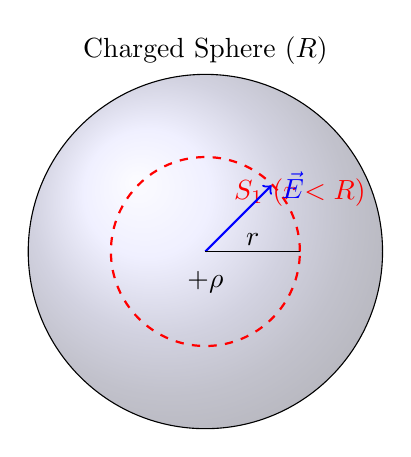
\begin{tikzpicture}[scale=1.5]
        % Sphere
        \shade[ball color=blue!20!white, opacity=0.4] (0,0) circle (1.5);
        \draw (0,0) circle (1.5);
        \node at (0,0) [label=below:{$+\rho$}] {};
        \node at (0, 1.7) {Charged Sphere ($R$)};
        % Gaussian surface inside
        \draw[red, dashed, thick] (0,0) circle (0.8);
        \node[red] at (0.8, 0.5) {$S_1$ ($r<R$)};
        % E-field vector inside
        \draw[->, thick, blue] (0,0) -- (0.56, 0.56) node[right]{$\vec{E}$};
        \draw (0,0) -- (0.8,0);
        \node at (0.4, 0.1) {$r$};
    \end{tikzpicture}
    \captionof{figure}{A spherical Gaussian surface $S_1$ inside a uniformly charged sphere is used to find the E-field at a distance $r < R$.}
\end{center}

\textbf{Key Result: E-field inside a uniformly charged sphere}\\
For a sphere of radius $R$ and uniform charge density $\rho$, the electric field at a distance $r < R$ from the center is:
$$ E = \frac{\rho r}{3\epsilon_0} $$
The force on a particle with charge $-q$ inside is $F = (-q)E = -\frac{q\rho}{3\epsilon_0}r$. This is a restoring force ($F \propto -r$), which leads to Simple Harmonic Motion (SHM).

\subsection{Electrostatics in Mechanics (\SI{25}{min})}
\subsubsection{Static Equilibrium}
For a body to be in equilibrium, two conditions must be met:
\begin{enumerate}
    \item \textbf{Net force is zero:} $\sum \vec{F} = 0$
    \item \textbf{Net torque is zero:} $\sum \vec{\tau} = 0$ (about any pivot)
\end{enumerate}

\subsubsection{Simple Harmonic Motion (SHM)}
SHM occurs when an object experiences a restoring force directly proportional to its displacement from equilibrium: $F = -kx$. This leads to oscillations with an angular frequency $\omega$ and period $T$:
$$ \omega = \sqrt{\frac{k}{m}} \quad \text{and} \quad T = \frac{2\pi}{\omega} $$

\newpage
\section{Olympiad Problem Walkthroughs}

\subsection{Problem 1: Rod in an Electric Field (SPhO 2023)}
\textit{A thin rod AB of length \SI{60}{cm} is suspended by two identical springs ($k=\SI{20}{\newton\per\meter}$) in a uniform downward E-field ($E=\SI{24}{\volt\per\meter}$). The linear charge density is $\lambda = 0.9x$ (in \si{\coulomb\per\meter} with $x$ in \si{\meter}). Find the inclination $\theta$ of the rod.}

\begin{center}
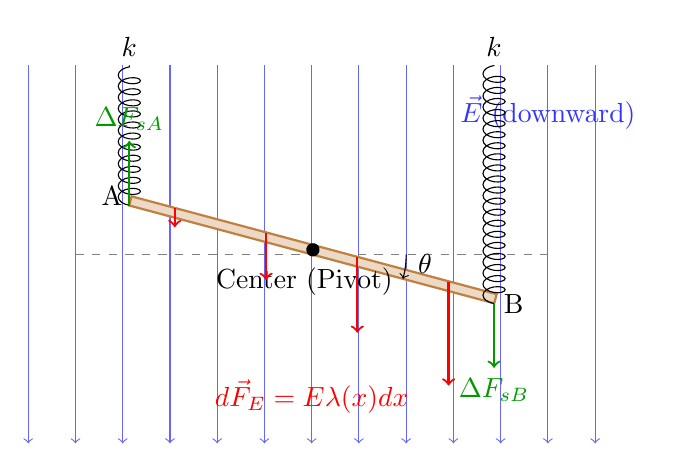
\begin{tikzpicture}[scale=1.2]
    % Electric field
    \foreach \x in {-3,-2.5,...,3} {
        \draw[->, blue!60, thin] (\x, 2) -- (\x, -2);
    }
    \node[blue!80] at (2.5, 1.5) {$\vec{E}$ (downward)};
    % Horizontal reference line
    \draw[dashed, gray] (-2.5, 0) -- (2.5, 0);
    % Tilted rod
    \begin{scope}[rotate=-15]
        \draw[thick, brown, fill=brown!30] (-2, 0) rectangle (2, 0.1);
        \node at (-2.2, 0.05) {A};
        \node at (2.2, 0.05) {B};
        \node at (0, -0.3) {Center (Pivot)};
        \fill (0, 0.05) circle (2pt);
    \end{scope}
    % Angle theta
    \draw[->] (1,0) arc (0:-15:1);
    \node at (1.2, -0.1) {$\theta$};
    % Springs
    \draw[decoration={coil,aspect=0.5,segment length=4pt,amplitude=4pt},decorate] (-1.93, 0.52) -- (-1.93, 2);
    \node at (-1.93, 2.2) {$k$};
    \draw[decoration={coil,aspect=0.5,segment length=4pt,amplitude=4pt},decorate] (1.93, -0.52) -- (1.93, 2);
    \node at (1.93, 2.2) {$k$};
    % Forces
    \draw[->, thick, green!60!black] (-1.93, 0.52) -- (-1.93, 1.2) node[above] {$\Delta F_{sA}$};
    \draw[->, thick, green!60!black] (1.93, -0.52) -- (1.93, -1.2) node[below] {$\Delta F_{sB}$};
    % Electric Force (non-uniform)
    \foreach \x in {-1.5, -0.5, 0.5, 1.5} {
        \pgfmathsetmacro{\force}{0.2 + 0.3*(\x+1.5)}
        \pgfmathsetmacro{\xcoord}{\x*cos(-15)}
        \pgfmathsetmacro{\ycoord}{\x*sin(-15)+0.1}
        \draw[->, thick, red] (\xcoord, \ycoord) -- (\xcoord, \ycoord-\force);
    }
    \node[red] at (0, -1.5) {$d\vec{F}_E = E\lambda(x)dx$};
\end{tikzpicture}
\captionof{figure}{Free-body diagram for the tilted rod in equilibrium.}
\end{center}

\textbf{Solution Strategy:} We balance the torques about the center of the rod.
\begin{enumerate}
    \item \textbf{Electric Torque ($\tau_E$):}
    \begin{align*}
        \tau_E = \int_0^L (x - L/2) (E \lambda(x) \cos\theta) \,dx = 21.6 \cos\theta \frac{L^3}{12}
    \end{align*}
    With $L = \SI{0.60}{m}$, $\tau_E = 0.3888 \cos\theta$ (clockwise).

    \item \textbf{Spring Torque ($\tau_S$):}
    $$ \tau_S = k \frac{L^2}{2} \sin\theta \cos\theta $$
    With $k=\SI{20}{\newton\per\meter}$ and $L = \SI{0.60}{m}$, $\tau_S = 3.6 \sin\theta \cos\theta$ (counter-clockwise).

    \item \textbf{Equilibrium:} Set $\tau_E = \tau_S$:
    \begin{align*}
        0.3888 \cos\theta = 3.6 \sin\theta \cos\theta \implies \sin\theta = \frac{0.3888}{3.6} = 0.108 \implies \theta \approx \SI{6.2}{\degree}
    \end{align*}
\end{enumerate}

\hrulefill
\subsection{Problem 2: Point Charges in a Rectangle (SPhO 2021)}
\textit{A rectangle has sides \SI{5.0}{cm} and \SI{15}{cm}. Arrangement: $q_1 = \SI{-5.0}{\micro\coulomb}$ (top left), A (top right), B (bottom left), $q_2 = \SI{+2.0}{\micro\coulomb}$ (bottom right).}

\begin{center}
    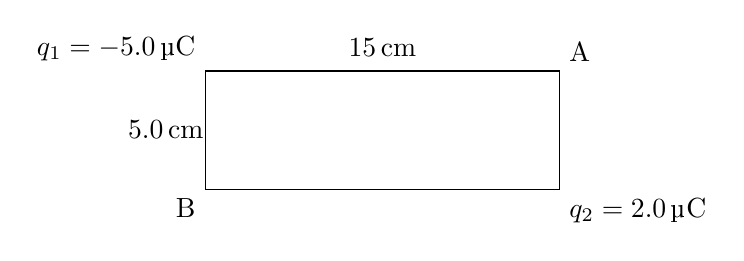
\begin{tikzpicture}
        \draw (0,1.5) -- (4.5,1.5) -- (4.5,0) -- (0,0) -- (0,1.5);
        \node at (0,1.5) [above left] {$q_1=\SI{-5.0}{\micro\coulomb}$};
        \node at (4.5,1.5) [above right] {A};
        \node at (0,0) [below left] {B};
        \node at (4.5,0) [below right] {$q_2=\SI{+2.0}{\micro\coulomb}$};
        \node at (2.25, 1.8) {\SI{15}{cm}};
        \node at (-0.5, 0.75) {\SI{5.0}{cm}};
    \end{tikzpicture}
    \captionof{figure}{The corrected arrangement of charges and points.}
\end{center}

Let $k = \dfrac{1}{4\pi\epsilon_0} \approx \SI{9.0e9}{\newton\meter\squared\per\coulomb\squared}$.

\begin{enumerate}
    \item[(a)] \textbf{Potential at corner A:} $r_{1A} = \SI{0.15}{m}$, $r_{2A} = \SI{0.05}{m}$.
    \begin{align*}
        V_A &= (\SI{9.0e9}{\newton\meter\squared\per\coulomb\squared}) \left( \frac{\num{-5.0e-6}}{\SI{0.150}{\meter}} + \frac{\num{2.0e-6}}{\SI{0.050}{\meter}} \right) \si{\coulomb} \\
        &= \SI{9.0e9}{} \left( -3.333\times10^{-5} + 4.000\times10^{-5} \right) \si{\volt} \\
        &= \SI{+6.00e4}{\volt}
    \end{align*}

    \item[(b)] \textbf{Potential at corner B:} $r_{1B} = \SI{0.05}{m}$, $r_{2B} = \SI{0.15}{m}$.
    \begin{align*}
        V_B &= (\SI{9.0e9}{\newton\meter\squared\per\coulomb\squared}) \left( \frac{\num{-5.0e-6}}{\SI{0.050}{\meter}} + \frac{\num{2.0e-6}}{\SI{0.150}{\meter}} \right) \si{\coulomb} \\
        &= \SI{9.0e9}{} \left( -1.000\times10^{-4} + 1.333\times10^{-5} \right) \si{\volt} \\
        &= \SI{-7.80e5}{\volt}
    \end{align*}

    \item[(c)] \textbf{Work to move $q_3 = \SI{+3.0}{\micro\coulomb}$ from B to A:}
    \begin{align*}
        W_{B \to A} &= q_3 (V_A - V_B) \\
        &= (\SI{3.0e-6}{\coulomb}) (\SI{+6.00e4}{\volt} - (\SI{-7.80e5}{\volt})) \\
        &= (\SI{3.0e-6}{\coulomb}) (\SI{8.40e5}{\volt}) = \SI{+2.52}{\joule}
    \end{align*}

    \item[(d)] The work done by the external agent is positive. This means the system's electric potential energy \textbf{increases}.
    
    \item[(e) \& (f)] The electrostatic force is conservative. Therefore, the work done is \textbf{the same} because it is path-independent.
\end{enumerate}

\hrulefill
\subsection{Problem 3: Merging Oil Drops (SPhO 2019)}
\textit{Two identical spherical oil drops with surface potential \SI{1000}{V} unite to form a single drop. What is the potential of the new drop?}

\begin{enumerate}
    \item \textbf{Initial State:} For one drop with charge $Q_1$ and radius $R_1$:
    $$ V_1 = \frac{k Q_1}{R_1} = \SI{1000}{V} $$
    
    \item \textbf{Conservation Laws:} When the drops merge:
    \begin{itemize}
        \item New charge: $Q_2 = 2Q_1$
        \item New volume: $V_{\text{vol,2}} = 2 V_{\text{vol,1}}$
    \end{itemize}
    
    \item \textbf{Find New Radius ($R_2$):}
    \begin{align*}
        \frac{4}{3}\pi R_2^3 &= 2 \times \frac{4}{3}\pi R_1^3 \\
        R_2^3 &= 2 R_1^3 \implies R_2 = 2^{1/3} R_1
    \end{align*}

    \item \textbf{Calculate New Potential ($V_2$):}
    \begin{align*}
        V_2 &= \frac{k Q_2}{R_2} = \frac{k(2Q_1)}{2^{1/3}R_1} = 2^{2/3} \left( \frac{kQ_1}{R_1} \right) \\
        V_2 &= 2^{2/3} V_1 = 2^{2/3} (\SI{1000}{V}) \approx \num{1.5874} \times \SI{1000}{V} = \SI{1587}{V}
    \end{align*}
\end{enumerate}

\hrulefill
\subsection{Problem 4: Particle in a Sphere Tunnel (SPhO 2020 \& 2023)}
\textit{A particle ($m$, $-q$) is released in a tunnel through a sphere (radius $R$, density $\rho$).}

\begin{enumerate}
    \item \textbf{Equation of Motion:} The E-field inside the sphere at distance $r$ is $E = \dfrac{\rho r}{3\epsilon_0}$. The force on charge $-q$ is:
    $$ F = (-q)E = -\left(\frac{q\rho}{3\epsilon_0}\right)r $$
    This is SHM, where the effective spring constant is $k_{\text{eff}} = \dfrac{q\rho}{3\epsilon_0}$.
    
    \item \textbf{Description of Motion:} The particle undergoes \textbf{Simple Harmonic Motion (SHM)} about the center of the sphere with an amplitude of $R$.
    
    \item \textbf{Calculations (SPhO 2023):}
    
    Given: $R=\SI{0.50}{m}$, $\rho = \SI{5.0}{\nano\coulomb\per\meter\cubed} = \SI{5.0e-9}{\coulomb\per\meter\cubed}$, $m=\SI{1.0}{\micro\gram} = \SI{1.0e-9}{kg}$, $q = \SI{0.05}{\nano\coulomb} = \SI{5.0e-11}{C}$.
    \begin{itemize}
        \item Angular frequency:
        \begin{align*}
            \omega &= \sqrt{\frac{q\rho}{3\epsilon_0 m}} \\
            &= \sqrt{\frac{(\num{5.0e-11})(\num{5.0e-9})}{3(\num{8.85e-12})(\num{1.0e-9})}} \\
            &\approx \sqrt{9.416} \approx \SI{3.07}{\radian\per\second}
        \end{align*}
        \item Time to cross the tunnel is half a period ($T/2$):
        $$ T = \frac{2\pi}{\omega} \approx \SI{2.05}{s} \implies t = \frac{T}{2} \approx \SI{1.02}{s} $$
        \item Speed at the center is the maximum speed in SHM ($v_{\text{max}} = A\omega$):
        $$ v_{\text{center}} = R\omega = (\SI{0.50}{m})(\SI{3.07}{\radian\per\second}) \approx \SI{1.54}{\meter\per\second} $$
    \end{itemize}
    \item \textbf{Speed Calculation (SPhO 2020):} In terms of variables, the speed is:
    $$ v_{\text{center}} = R\sqrt{\frac{q\rho}{3\epsilon_0 m}} $$
\end{enumerate}

\hrulefill
\subsection{Problem 5: Charged Object on Ring Axis (SPhO 2022)}
\textit{A ring ($R=\SI{50}{cm}, \lambda = \SI{+10}{\nano\coulomb\per\meter}$) and an object ($m=\SI{1}{mg}, q=\SI{-5.0}{\nano\coulomb}$) starting at $x_0 = \SI{5.0}{mm}$.}

\begin{enumerate}
    \item \textbf{Approximation for SHM:} The E-field on the axis is $E_x = \dfrac{kQx}{(R^2+x^2)^{3/2}}$.
    Since $x_0 \ll R$, we approximate $(R^2+x^2)^{3/2} \approx R^3$.
    $$ E_x \approx \frac{kQ}{R^3}x $$
    The force on charge $q$ is $F_x = qE_x \approx -\frac{k|q|Q}{R^3}x$. This is SHM with $k_{\text{eff}} = \dfrac{k|q|Q}{R^3}$.
    
    \item[(a)] \textbf{Time to reach the center:} This time is one-quarter of a period ($T/4$).
    \begin{itemize}
        \item Total charge on ring: $Q = \lambda(2\pi R) = (\SI{10e-9}{\coulomb\per\meter})(2\pi \times \SI{0.50}{m}) = \num{3.142e-8} \si{\coulomb}$.
        \item Effective spring constant:
        \begin{align*}
            k_{\text{eff}} &= \frac{(\num{9.0e9})(\num{5.0e-9})(\num{3.142e-8})}{(\num{0.50})^3} \\
            &= \frac{\num{1.414e-6}}{0.125} \approx \SI{1.131e-5}{\newton\per\meter}
        \end{align*}
        \item Angular frequency: $\omega = \sqrt{\frac{k_{\text{eff}}}{m}} = \sqrt{\frac{\SI{1.131e-5}{\newton\per\meter}}{\SI{1.0e-6}{kg}}} \approx \SI{3.36}{\radian\per\second}$.
        \item Period: $T = \frac{2\pi}{\omega} \approx \SI{1.87}{s}$.
        \item Time to center: $t = T/4 \approx \SI{0.468}{s}$.
    \end{itemize}

    \item[(b)] \textbf{Kinetic Energy at the center:} Use conservation of energy. $K_f = -q(V(0) - V(x_0))$.
    The potential on the axis is $V(x) = \dfrac{kQ}{\sqrt{R^2+x^2}}$.
    \begin{align*}
        K_f &= -q \left( \frac{kQ}{R} - \frac{kQ}{\sqrt{R^2+x_0^2}} \right) \\
        &= (\SI{5.0e-9}{\coulomb}) \cdot (\num{9.0e9}) \cdot (\num{3.142e-8}) \left( \frac{1}{0.50} - \frac{1}{\sqrt{0.50^2 + 0.005^2}} \right) \\
        &= (\num{1.414e-6}) \left( 2.0000 - 1.9999 \right) \approx \SI{1.41e-10}{\joule}
    \end{align*}
\end{enumerate}

\newpage
\section{New Problems and Solutions}

\subsection{Problem A: Tilted Disc in an Electric Field}
\textit{A thin, non-conducting disc of radius $R = \SI{20}{cm}$ is pivoted at its center. The disc has a non-uniform surface charge density given by $\sigma = \sigma_0 \frac{r}{R} \cos^2\phi$, where $\sigma_0 = \SI{50}{\nano\coulomb\per\meter\squared}$. The disc is in a uniform downward electric field of $E = \SI{2000}{\volt\per\meter}$. A small mass $m = \SI{2}{g}$ is attached to the edge at $\phi = \ang{180}$. Find the angle $\theta$ that the x-axis of the disc makes with the horizontal at equilibrium.}

\begin{center}
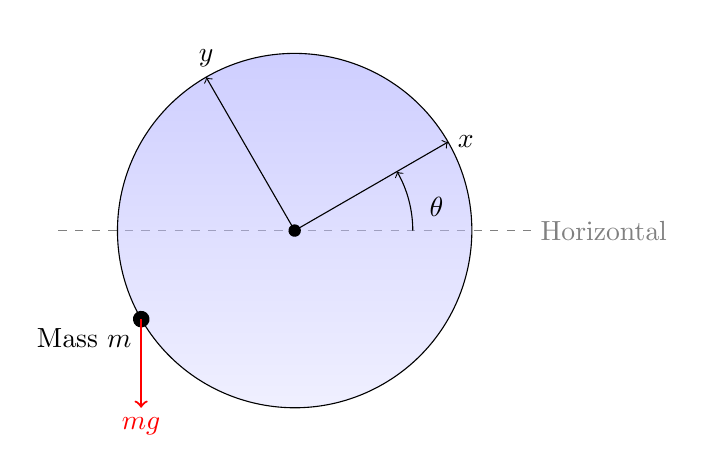
\begin{tikzpicture}[scale=1.5]
    % Horizontal line
    \draw[dashed, gray] (-2,0) -- (2,0) node[right] {Horizontal};
    
    % Tilted disc
    \begin{scope}[rotate=30]
        \shade[top color=blue!40, bottom color=blue!10, opacity=0.5] (0,0) circle (1.5cm);
        \draw (0,0) circle (1.5cm);
        \draw[->] (0,0) -- (1.5,0) node[right] {$x$};
        \draw[->] (0,0) -- (0,1.5) node[above] {$y$};
        \fill (0,0) circle (1.5pt);
        \node[below left] at (-1.5,0) {Mass $m$};
        \fill (-1.5,0) circle (2pt);
    \end{scope}
    
    % Angle
    \draw[->] (1,0) arc (0:30:1);
    \node at (1.2, 0.2) {$\theta$};
    
    % Gravity Force
    \draw[->, thick, red] (-1.3,-0.75) -- (-1.3, -1.5) node[below] {$mg$};
\end{tikzpicture}
\captionof{figure}{A charged disc with an attached mass, tilted by an angle $\theta$ in an electric field.}
\end{center}

\textbf{Explanation and Solution:}
The system is in equilibrium when the net torque about the pivot is zero.
\begin{enumerate}
    \item \textbf{Gravitational Torque ($\tau_g$):} The mass is at $r=R, \phi=\ang{180}$. When the disc tilts by $\theta$, its horizontal position is $-R\cos\theta$. The torque due to gravity is $\tau_g = (mg)(R\cos\theta)$, acting counter-clockwise (restoring).
    
    \item \textbf{Electric Torque ($\tau_E$):} The torque on a charge element $dQ=\sigma dA$ in a downward field $-E\hat{k}$ is $d\vec{\tau}_E = \vec{r} \times (-E\,dQ\,\hat{k})$. With $\vec{r} = r\cos\phi\,\hat{i} + r\sin\phi\,\hat{j}$, the torque component causing the tilt (rotation about the y-axis) is $d\tau_y = -E r \cos\phi \,dQ$.
    $$ \tau_E = \int_0^R \int_0^{2\pi} -E r \cos\phi \left( \sigma_0 \frac{r^2}{R} \cos^2\phi \right) dr\,d\phi = -\frac{E\sigma_0}{R} \int_0^R r^3 dr \int_0^{2\pi} \cos^3\phi \, d\phi $$
    Since $\int_0^{2\pi} \cos^3\phi \,d\phi = 0$, the net electric torque is \textbf{zero}. The charge distribution is symmetric and does not cause a tilt.
    
    \item \textbf{Equilibrium:} The equilibrium is determined only by the mass.
    $$ \tau_{\text{net}} = \tau_g = mgR\cos\theta = 0 \implies \cos\theta = 0 $$
    Therefore, the disc tilts until the mass is at its lowest point, so $\theta = \ang{90}$.
\end{enumerate}

\hrulefill
\subsection{Problem B: Equilateral Triangle of Charges}
\textit{Three charges are at the vertices of an equilateral triangle (side $s = \SI{30}{cm}$): $q_1 = \SI{+4.0}{\micro\coulomb}$, $q_2 = \SI{+4.0}{\micro\coulomb}$, and $q_3 = \SI{-2.0}{\micro\coulomb}$. Let A be the midpoint between $q_1, q_2$ and B be the centroid. (a) Find the potential at A and B. (b) Find the work to move an electron from A to B.}

\begin{center}
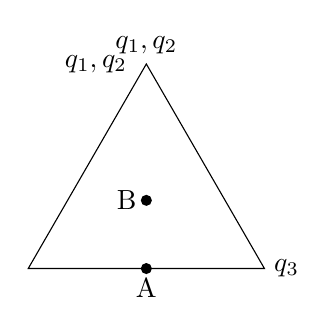
\begin{tikzpicture}
    % Triangle
    \coordinate (Q1) at (0, 2.598);
    \coordinate (Q2) at (-1.5, 0);
    \coordinate (Q3) at (1.5, 0);
    \draw (Q1) -- (Q2) -- (Q3) -- cycle;
    
    % Charges and Points
    \node at (Q1) [above] {$q_1, q_2$}; % Simplified for diagram
    \node at (Q3) [right] {$q_3$};
    \node at (0,0) [below] {A};
    \node at (0, 0.866) [left] {B};
    \fill (0,0) circle (2pt);
    \fill (0, 0.866) circle (2pt);
    \node at (Q1) [label=left:{$q_1, q_2$}] {}; % for clarity
\end{tikzpicture}
\captionof{figure}{Configuration of charges on an equilateral triangle.}
\end{center}

\textbf{Explanation and Solution:}
(a) The height of the triangle is $h = s\sin(60^\circ) \approx \SI{0.2598}{m}$. The centroid B is at $1/3$ the height, so its distance to each vertex is $d_B = s/\sqrt{3} \approx \SI{0.1732}{m}$.
\begin{itemize}
    \item \textbf{Potential at A:} Distances are $s/2 = \SI{0.15}{m}$ (to $q_1, q_2$) and $h$ (to $q_3$).
\begin{align*} 
V_A &= (9 \times 10^9) \left( \frac{\SI{4e-6}{\coulomb}}{\SI{0.15}{\meter}} \times 2 + \frac{\SI{-2e-6}{\coulomb}}{\SI{0.2598}{\meter}} \right) = \SI{4.11e5}{\volt} 
\end{align*}

\item \textbf{Potential at B:} Distance to all charges is $d_B = \SI{0.1732}{\meter}$.
\begin{align*} 
V_B &= \frac{9 \times 10^9}{\SI{0.1732}{\meter}} (\SI{4e-6}{\coulomb} + \SI{4e-6}{\coulomb} - \SI{2e-6}{\coulomb}) = \SI{3.12e5}{\volt} 
\end{align*}
\end{itemize}
(b) Work to move an electron ($q_e = \SI{-1.602e-19}{C}$):
\begin{align*} W_{A \to B} &= q_e (V_B - V_A) = (\SI{-1.602e-19}{C}) (\SI{3.12e5}{V} - \SI{4.11e5}{V}) = \SI{1.59e-14}{J} \end{align*}

\hrulefill
\subsection{Problem C: Combining Charged Wires}
\textit{Two long, identical conducting wires ($L = \SI{1}{m}, r_1 = \SI{1}{mm}$) are charged to a potential of $V_1 = \SI{5000}{V}$. They are merged into a single wire of the same length. Find the potential $V_2$ of the new wire.}

\textbf{Explanation and Solution:}
We use conservation of charge and the formula for capacitance of a single wire, $C = \frac{2\pi\epsilon_0 L}{\ln(L/r)}$.
\begin{enumerate}
    \item \textbf{Initial State:} $Q_1 = C_1 V_1 = \frac{2\pi\epsilon_0 L V_1}{\ln(L/r_1)}$.
    \item \textbf{Conservation:} Total charge is $Q_2 = 2Q_1$. Volume conservation ($L$ is constant) means cross-sectional area doubles: $A_2 = 2A_1 \implies \pi r_2^2 = 2\pi r_1^2 \implies r_2 = \sqrt{2}r_1$.
    \item \textbf{Final Potential:}
    $$ V_2 = \frac{Q_2}{C_2} = \frac{2Q_1}{ \frac{2\pi\epsilon_0 L}{\ln(L/r_2)} } = 2 V_1 \frac{\ln(L/(\sqrt{2}r_1))}{\ln(L/r_1)} $$
    $$ V_2 = 2(\SI{5000}{V}) \frac{\ln(1000/\sqrt{2})}{\ln(1000)} = \SI{10000}{V} \left( 1 - \frac{0.5\ln(2)}{\ln(1000)} \right) \approx \SI{9500}{V} $$
\end{enumerate}

\hrulefill
\subsection{Problem D: Particle Oscillating in a Charged Cylinder}
\textit{An infinitely long cylinder of radius $R$ has uniform charge density $\rho$. A narrow tunnel is drilled at a distance $d$ from the axis. A particle ($m, -q$) is released in the tunnel. Show it undergoes SHM and find its period.}

\begin{center}
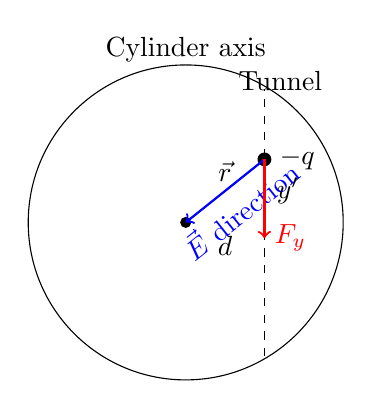
\begin{tikzpicture}
    % Cylinder cross-section
    \draw (0,0) circle (2cm);
    \node at (0, 2.2) {Cylinder axis};
    \fill (0,0) circle (2pt);
    
    % Tunnel
    \draw[dashed] (1,-1.7) -- (1,1.7);
    \node at (1.2, 1.8) {Tunnel};
    
    % Particle
    \coordinate (P) at (1, 0.8);
    \fill (P) circle (2.5pt) node[right=2pt] {$-q$};
    
    % Vectors
    \draw[->] (0,0) -- (P) node[midway, above] {$\vec{r}$};
    \draw[->, thick, blue] (P) -- (0,0) node[midway, below, sloped] {$\vec{E}$ direction};
    \draw[->, thick, red] (P) -- (1, -0.2) node[right] {$F_y$};
    \node at (0.5, -0.3) {$d$};
    \node at (1.3, 0.4) {$y'$};
\end{tikzpicture}
\captionof{figure}{Cross-section of the cylinder showing the restoring force on the particle.}
\end{center}

\textbf{Explanation and Solution:}
\begin{enumerate}
    \item \textbf{E-Field Inside Cylinder (from Gauss's Law):} For an infinite cylinder, the field at radius $r<R$ is purely radial: $E = \frac{\rho r}{2\epsilon_0}$.
    
    \item \textbf{Force on Particle:} The particle is at position $(d, y')$, so its distance from the axis is $r = \sqrt{d^2+y'^2}$. The force vector is $\vec{F} = -q\vec{E} = -q \frac{\rho}{2\epsilon_0} \vec{r} = -\frac{q\rho}{2\epsilon_0}(d\hat{i} + y'\hat{j})$.
    
    \item \textbf{SHM:} The particle is constrained to move along the tunnel (y-direction). The restoring force is the y-component:
    $$ F_y = -\left( \frac{q\rho}{2\epsilon_0} \right) y' $$
    This is in the form $F = -k_{\text{eff}}y'$, which defines SHM.
    
    \item \textbf{Period:} The period is $T = 2\pi\sqrt{m/k_{\text{eff}}}$.
    $$ T = 2\pi\sqrt{\frac{2m\epsilon_0}{q\rho}} $$
\end{enumerate}

\hrulefill
\subsection{Problem E: Oscillation Between Two Charges}
\textit{Two charges $+Q$ are fixed at $x = \pm a$. A particle ($m, +q$) is constrained to the y-axis. (a) Find its equilibrium position. (b) Show it undergoes SHM for small y-displacements. (c) Find its angular frequency.}

\begin{center}
\begin{tikzpicture}
    % Axes
    \draw[->] (-3,0) -- (3,0) node[below] {$x$};
    \draw[->] (0,-2) -- (0,2) node[left] {$y$};
    
    % Fixed charges
    \fill (-2,0) circle (2.5pt) node[below] {$-a, +Q$};
    \fill (2,0) circle (2.5pt) node[below] {$+a, +Q$};
    
    % Oscillating charge
    \coordinate (q) at (0,1);
    \fill (q) circle (2.5pt) node[right] {$+q$};
    
    % Force vectors
    \draw[->, thick, red] (q) -- (1.78, 0.447); % F from right charge
    \draw[->, thick, red] (q) -- (-1.78, 0.447); % F from left charge
    \draw[->, thick, blue, very thick] (q) -- (0, 1.89) node[above] {$F_{net}$};
\end{tikzpicture}
\captionof{figure}{Symmetry of forces on the charge $+q$ on the y-axis.}
\end{center}

\textbf{Explanation and Solution:}
\begin{enumerate}
    \item[(a)] \textbf{Equilibrium:} At $y=0$, the repulsive forces from the two $+Q$ charges are equal and opposite, so the net force is zero. The equilibrium position is the origin.
    
    \item[(b)] \textbf{Restoring Force:} At a small displacement $y$, the distance to each charge is $s=\sqrt{a^2+y^2}$. The net force is the sum of the y-components:
    $$ F_{net} = 2 \left( \frac{kQq}{a^2+y^2} \right) \sin\theta = 2 \frac{kQq}{(a^2+y^2)} \frac{y}{\sqrt{a^2+y^2}} = \frac{2kQqy}{(a^2+y^2)^{3/2}} $$
    For $y \ll a$, this simplifies to a restoring force:
    $$ F_{net} \approx \frac{2kQqy}{a^3} $$
    Since the force is directed away from equilibrium, we write $F \approx -\left(\frac{2kQq}{a^3}\right)y$. This is SHM.
    
    \item[(c)] \textbf{Angular Frequency:} From $F = -k_{\text{eff}}y$, we identify $k_{\text{eff}} = \frac{2kQq}{a^3}$.
    The angular frequency is:
    $$ \omega = \sqrt{\frac{k_{\text{eff}}}{m}} = \sqrt{\frac{2kQq}{ma^3}} $$
\end{enumerate}

\newpage
\section{Derivations of Key Formulas}

\subsection{Derivation for Problem 4: E-Field Inside a Uniform Sphere}
This derivation uses Gauss's Law: $\oint \vec{E} \cdot d\vec{A} = Q_{\text{enc}}/\epsilon_0$.
\begin{itemize}
    \item For a spherical Gaussian surface of radius $r<R$, the flux is $E(4\pi r^2)$.
    \item The enclosed charge is $Q_{\text{enc}} = \rho(\frac{4}{3}\pi r^3)$.
    \item Equating them gives $E(4\pi r^2) = \frac{\rho}{\epsilon_0}(\frac{4}{3}\pi r^3) \implies E = \frac{\rho r}{3\epsilon_0}$.
\end{itemize}

\subsection{Derivation for Problem 5: E-Field on the Axis of a Charged Ring}
This derivation uses integration and symmetry.
\begin{center}
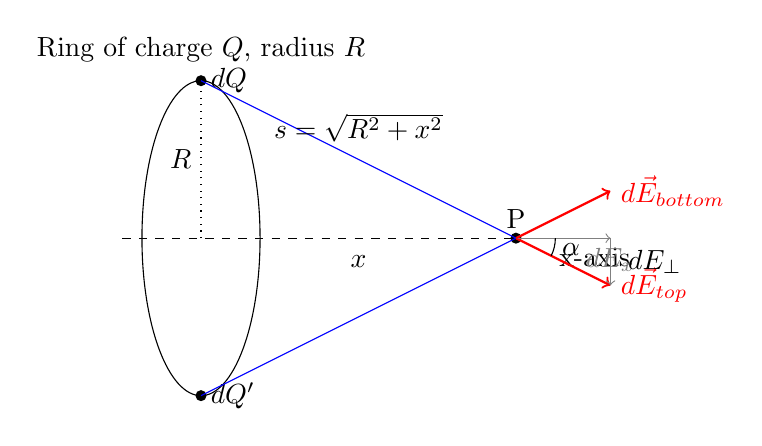
\begin{tikzpicture}
    % Ring in vertical plane
    \draw (0,0) ellipse (0.75cm and 2cm);
    \node at (0, 2.4) {Ring of charge $Q$, radius $R$};
    
    % Axis
    \draw[dashed] (-1,0) -- (5,0) node[below] {x-axis};
    
    % Point P
    \fill (4,0) circle (2pt) node[above] {P};
    \node at (2, -0.3) {$x$};
    
    % Charge element dQ at top
    \fill (0,2) circle (2pt) node[right] {$dQ$};
    
    % Line from dQ to P
    \draw[blue] (0,2) -- (4,0);
    \node at (2,1.4) {$s = \sqrt{R^2+x^2}$};
    
    % Radius R
    \draw[dotted] (0,0) -- (0,2) node[midway, left] {$R$};
    
    % dE vector from top element
    \draw[->, thick, red] (4,0) -- (5.2, -0.6) node[anchor=west] {$d\vec{E}_{top}$};
    
    % dE_x component
    \draw[->, gray] (4,0) -- (5.2,0) node[below] {$dE_x$};
    
    % dE_perp component (downwards)
    \draw[->, gray] (5.2,0) -- (5.2, -0.6);
    \node at (5.3, -0.3) [right] {$dE_\perp$};
    
    % Charge element dQ at bottom
    \fill (0,-2) circle (2pt) node[right] {$dQ'$};
    \draw[blue] (0,-2) -- (4,0);
    
    % dE vector from bottom element
    \draw[->, thick, red] (4,0) -- (5.2, 0.6) node[anchor=west] {$d\vec{E}_{bottom}$};
    
    % Angle alpha
    \begin{scope}[shift={(4,0)}]
        \draw (0,0) ++ (0.5,0) arc (0:-26.5:0.5);
        \node at (0.7,-0.15) {$\alpha$};
    \end{scope}
\end{tikzpicture}
\captionof{figure}{By symmetry, perpendicular field components cancel, leaving only x-components.}
\end{center}
\begin{itemize}
    \item The field from an element $dQ$ is $dE = \frac{k dQ}{R^2+x^2}$.
    \item By symmetry, only the x-components sum up: $dE_x = dE \cos\alpha$.
    \item From geometry, $\cos\alpha = \frac{x}{\sqrt{R^2+x^2}}$.
    \item Integrating gives $E_x = \int dE_x = \int \frac{k x}{(R^2+x^2)^{3/2}} dQ = \frac{k Q x}{(R^2+x^2)^{3/2}}$.
\end{itemize}

\end{document}